\subsection{Virtual PTZ camera}
Initially, some simple transformations were carried out in MatLab using a symmetrical set of normalized homogeneous points, i.e. four points with coordinates (-1,-1,1), (1,-1,1), (1,1,1) and (-1,1,1) in $\mathbb{P}^2$.

Secondary trials were made with a point set with origo in a corner point, similar to the coordinate system in an image. Here ``calibration'' matrices were needed in order to move the image origo to the center of the image and scale it.

Advancments into real-images were then straight forward as the synthezised calibration matrices were replaced with the real calibration matrices.

Actual implementation in c++ in combination with the stiching homographies were initially troublesome, but as it was soon realized that first applying stiching homographies and then applying the PTZ-transform made the images keep the correct relations to each other. The were also some problems with the PTZ-transform being applied twice on some of the stiched images, giving the impression that parts of the scene were ``drifting'' away, as well as the image masks not being transformed the same way as the images themselves.

These issues were however solved and an example of the resulting ptz movement can be seen in fig. \ref{fig:ptz_res}.

\begin{figure}[H]
	\centering
	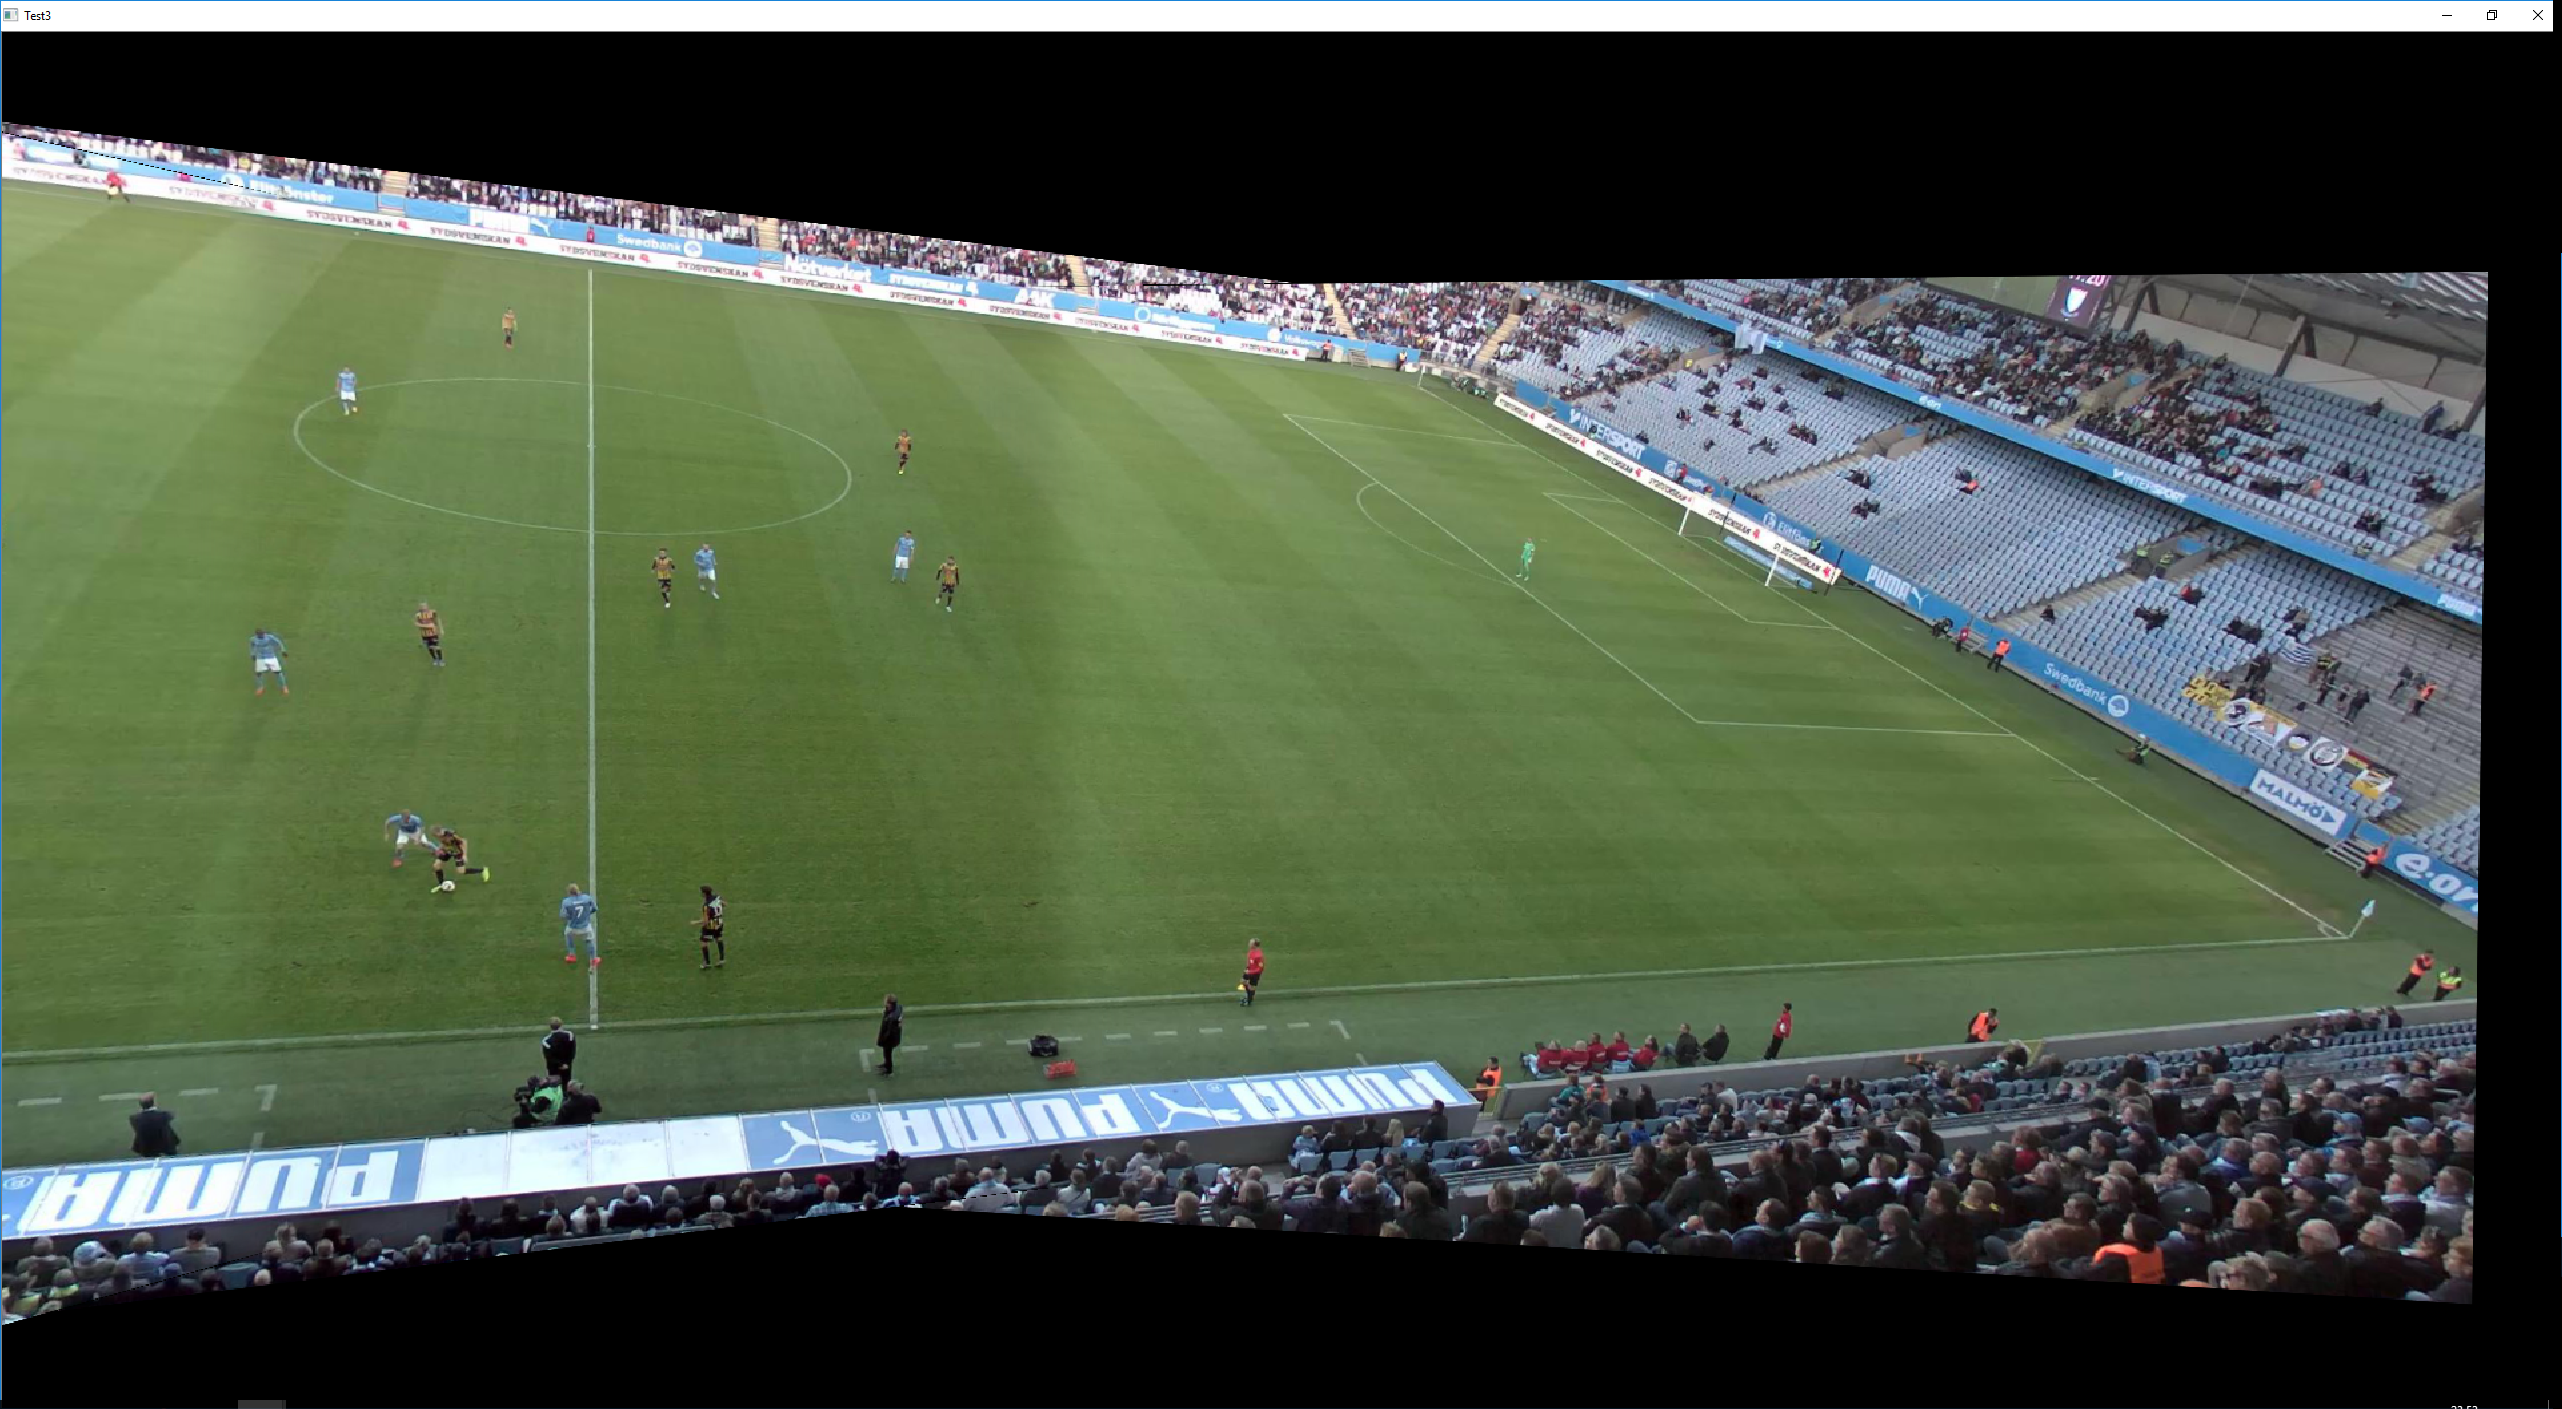
\includegraphics[width=0.8\columnwidth]{../results/images/PTZ_res.PNG}
	\caption{An example of the resulting image where the virtual camera has been panned, tilted and zoomed.}
	\label{fig:ptz_res}
\end{figure}
